\chapter{Background on Convolutional Neural Networks}\label{ch:cnn}
Convolutional neural networks (CNNs) have been one of the most influential innovations in the field of computer vision. Neural networks became popular in 2012 when Alex Krizhevsky used them to win that year's ImageNet competition\cite{aleximagenet} by dropping the error from 26\% to 15\%. Since then, many companies are using deep learning including Facebook's tagging algorithms, Google for their photo search and Amazon for product recommendations. For the purpose of this thesis CNNs were used for image classification, specifically, images of varying particles created using LArTPC data. 

\section{Image Classification} 
Image classification is the process of inputting an image into the CNN an receiving a probability of classes that best describes what is happening in the image. As humans, image classification is something that is learned at a very young age and is easy to do without much effort. This is also apparent when hand-scanning LArTPC images. After learning what a neutrino event looks like in MicroBooNE, it is relatively easy to recognize simple neutrino events from cosmic ray background as well as highly ionizing particles like protons from minimum ionizing particles like muons. The very detailed images LArTPC detectors output are prime candidates for input images into a CNN. CNNs mimic a human's ability to classify objects by creating an architecture that can learn differences between all the images it's given as well as figure out the unique features that make up each object. CNNs are modeled after the visual cortex. Hubel and Wiesel\cite{hubel} found that there are small regions of neuronal cells in the brain that respond to specific regions of the visual field. They saw that some neurons fired when exposed to vertical edges while others fired when shown horizontal or diagonal edges. They also saw that these neurons were organized in columns. The idea of specific neurons inside of the brain firing to specific characteristics is the basis behind CNNs.

\subsection{CNN Structure}
When used for image recognition, convolutional neural networks consist of multiple layers that extract different information on small portions of the input image. How many layers is tunable to increase the accuracy. The output of these collections are then tiled so that they overlap to gain a better representation of the original image and allow for translation. The first of these layers is always a convolution layer. To the CNN, an image is an array of pixel values. For a RGB color image with width and height equal to 32x32 the corresponding array is 32x32x3. Filters, also known as neurons, of any size set by the user is then convolved with the receptive field of the image. If the filter is 5x5, the receptive field will by a patch of 5x5 on the input image. The filter is also an array of numbers called weights. The convolution of the filter and image are matrix multiplications of the weights and the pixel values. By stepping the receptive field by 1 unit, for an input image of 32x32x3 and a filter of 5x5x3 you'd get an output array of 28x28x1. This output array is called an activation map or feature map. The use of more filters preserves the spatial dimensions better. The filters can be described as feature identifiers. Examples of features in an image consist of edges, curves, and changes in colors. The first filters in a CNN will primarily be straight line and curve feature identifiers. An example of a curve filter is shown in figure \ref{fig:curvedetector}. When a curve in the same concavity is found in the input image, the corresponding pixel in the output feature map will be activated. Going back to our example of a 32x32 input image and a 5x5 filter, if there were to be a curve in the top left corner of the input image, our output feature map would have a high pixel value in the top left. Therefore, feature maps tell us where a specific feature is located in the original image. Figure \ref{fig:conv1} shows a visualization of filters found in the first layers of many CNN architectures. These filters in the first layer convlove around the image and activate whe nthe specific feature it is looking for is in the receptive field. 
\begin{figure}[htp!]
\centering
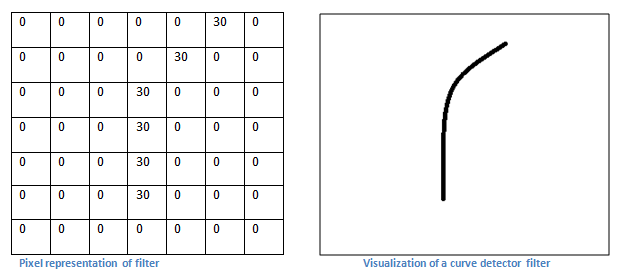
\includegraphics[width=.6\textwidth]{figs/curvedetector.png}
\caption{Pixel representation and visualization of a curve detector filter. As you can see, in the pixel representation, the weights of this filter are greater along a curve we are trying to find in the input image}
\label{fig:curvedetector}
\end{figure} 

\begin{figure}[htp!]
\centering
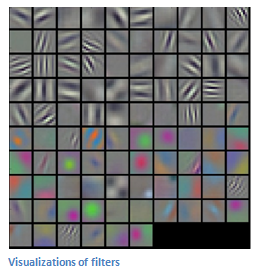
\includegraphics[width=.25\textwidth]{figs/conv1vis.png}
\caption{Visualization of filters found in first layer of a CNN.}
\label{fig:curvedetector}
\end{figure} 

In figure \ref{fig:convolution} you can see how an edge detection filter is used to save only necessary information for recognizing different types of clothes. You can also see by having multiple filters you can get more detail or less detail from an image which can then simplify or complicate the object recognition task. Being able to distinguish between a shirt or a leg garment is as much information you want, having a filter that extracts outline edge or shape information would be all that you need. But if instead you wanted to distinguish between a formal cocktail dress or a summer dress, more information would need to be saved equating to many more filters for one image. Rather than trying to come up with how many filters and what features are important for detection, CNNs do this automatically. CNNs take input parameters, called hyper-parameters, for example number of layers, number of filters per layers, number of weights per filter, and uses these to create the output feature maps. The layers build upon each-other, for example if we were creating a CNN for facial recognition the convolutional layers will start learning feature combinations off of the previous layers. The simple edges, gradients, and corners of the first layers become things like eyes, noses, and hairs in later layers. This process is visualized in figure \ref{fig:featuremaps} 

\begin{figure}[t!]
\centering
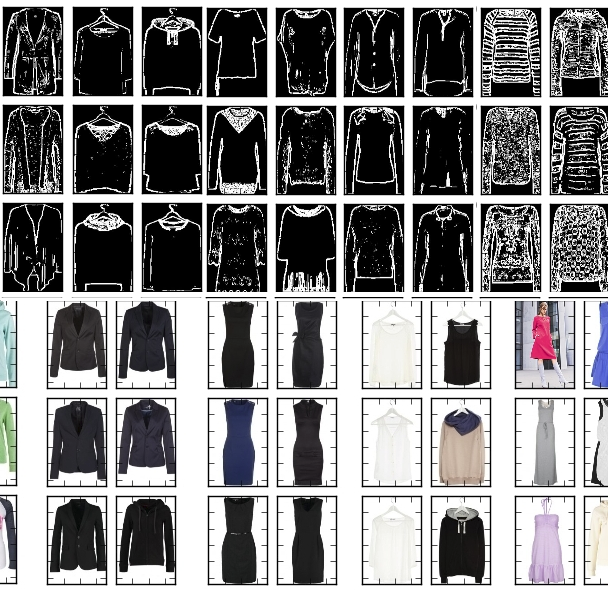
\includegraphics[width=.48\linewidth]{figs/convolution.png}
\caption{Applying a feature mask over a set of fashion items to extract necessary information for auto-encoding. Unnecessary information for example color or brand emblems are not saved. This feature map is an edge detection mask that leaves only shape information which helps to distinguish between different types of clothes.} 
\label{fig:convolution}
\end{figure}

\begin{figure}[h!]
\centering
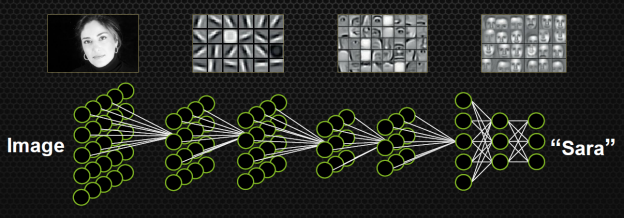
\includegraphics[width=.9\linewidth]{figs/facialDetection.png}
\caption{Pictorial Representation of Convolutional Neural Networks as well as a visual representation on CNN's complexity of layer feature extraction}
\label{fig:featuremaps}
\end{figure}
There are other layers in a CNN architecture that will not be covered in the scope of this thesis but in a general sense, these layers are interspersed between convolution layers to preserve dimensionality and control overfitting of the network. The last layer is called a fully connected layer and it's job is to output an N dimensional vector where N is the number of classes the network has been trained on. Each number in this vector represents the probability that the input image is a certain class. Fully connected layers use the feature maps of the high level features to compute the products between the weights of the previous layer to get the probabilites of each class. These weights are then adjusted throught the training process using backpropagation. 
\section{AlexNet}
\section{GoogleNet}
